\section{Introduction}
As introduced in chapter \ref{ch:robot}, point cloud is a data structure used to represent a collection of multi-dimensional points and is commonly used to represent three-dimensional data. In a 3D point cloud, the points usually represent the X, Y, and Z geometric coordinates of an underlying sampled surface. When color information is present, the point cloud becomes 4D. Point clouds can be acquired from hardware sensors such as stereo cameras, 3D scanners, or time-of-flight cameras, or generated from a computer program synthetically, \citet{pclib}.
In the scope of this thesis, Realsense camera D455 was used in order to perform point cloud generation that was in turn used to generate the occupancy grid of the space around the robot.
In figure \ref{table:camerasCharacteristics} are reported the features of D455 camera.

\begin{table}[H]
    \centering 
\begin{tabular}{|c|c|}
\hline
\textbf{Sensor Technology} & Global Shutter    \\ \hline
\textbf{Ideal Range}       & from 0.6 m to 6 m \\ \hline
\textbf{Depth} &
  \begin{tabular}[c]{@{}c@{}}Technology: Stereoscopic\\ Field of View: 87° x 58°\\ Output Resolution: up to 1280 × 720\\ Accuracy: \textless 0.02 m at 4 m \\ Frame rate: up to 90 fps\end{tabular} \\ \hline
\textbf{RGB} &
  \begin{tabular}[c]{@{}c@{}}Technology: Global Shutter\\ Field of View: 90°×65°\\ Output Resolution: up to 1280×800\\ Sensor Resolution: 1 MP\\ Frame rate: up to 30 fps\end{tabular} \\ \hline
\end{tabular}
    \\[10pt]
    \caption{Highlighted camera's specifications.}
    \label{table:camerasCharacteristics}
\end{table}

\begin{figure}[H]
\centering
\begin{tabular}{cc}
\subfloat[]{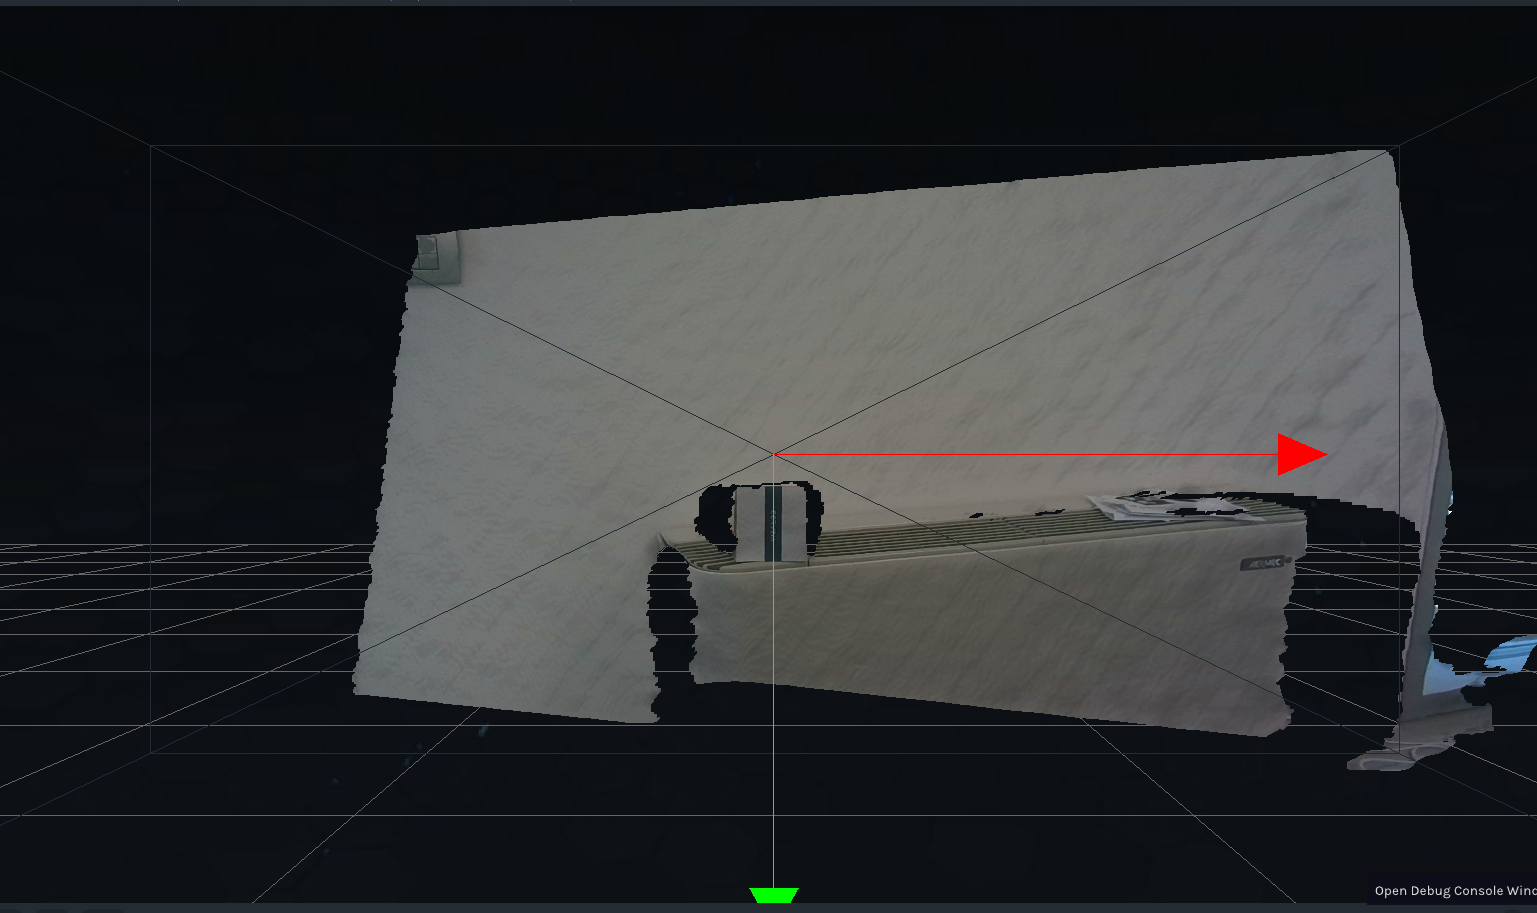
\includegraphics[width = 3in]{Images/Chapter 6/pcl1.png}}&
\subfloat[]{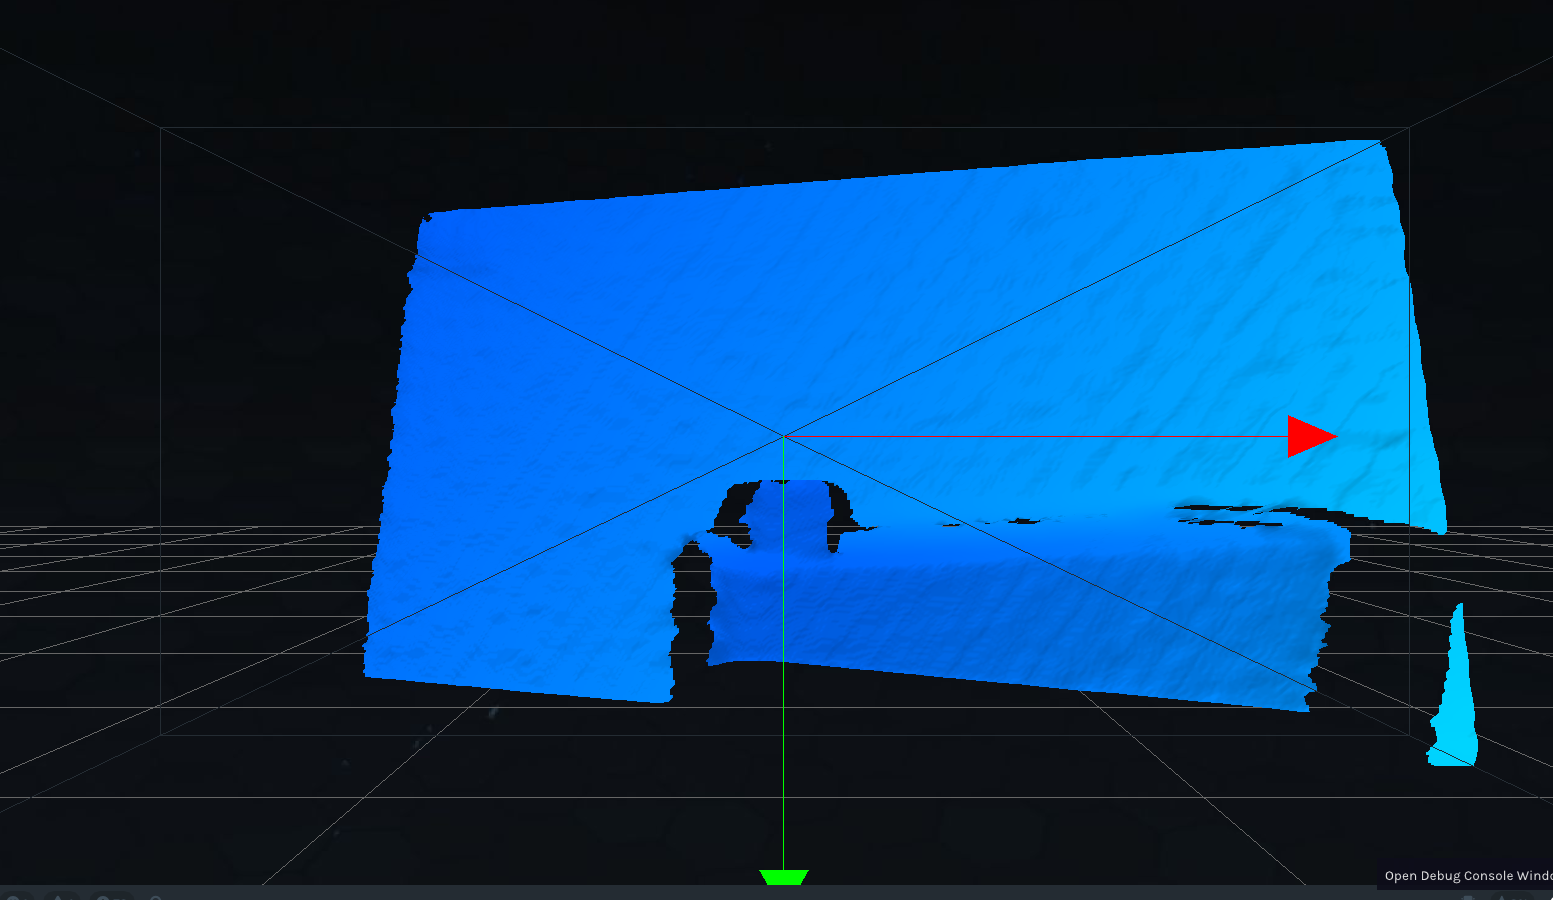
\includegraphics[width = 3in]{Images/Chapter 6/rgbd1.png}}\\
\subfloat[]{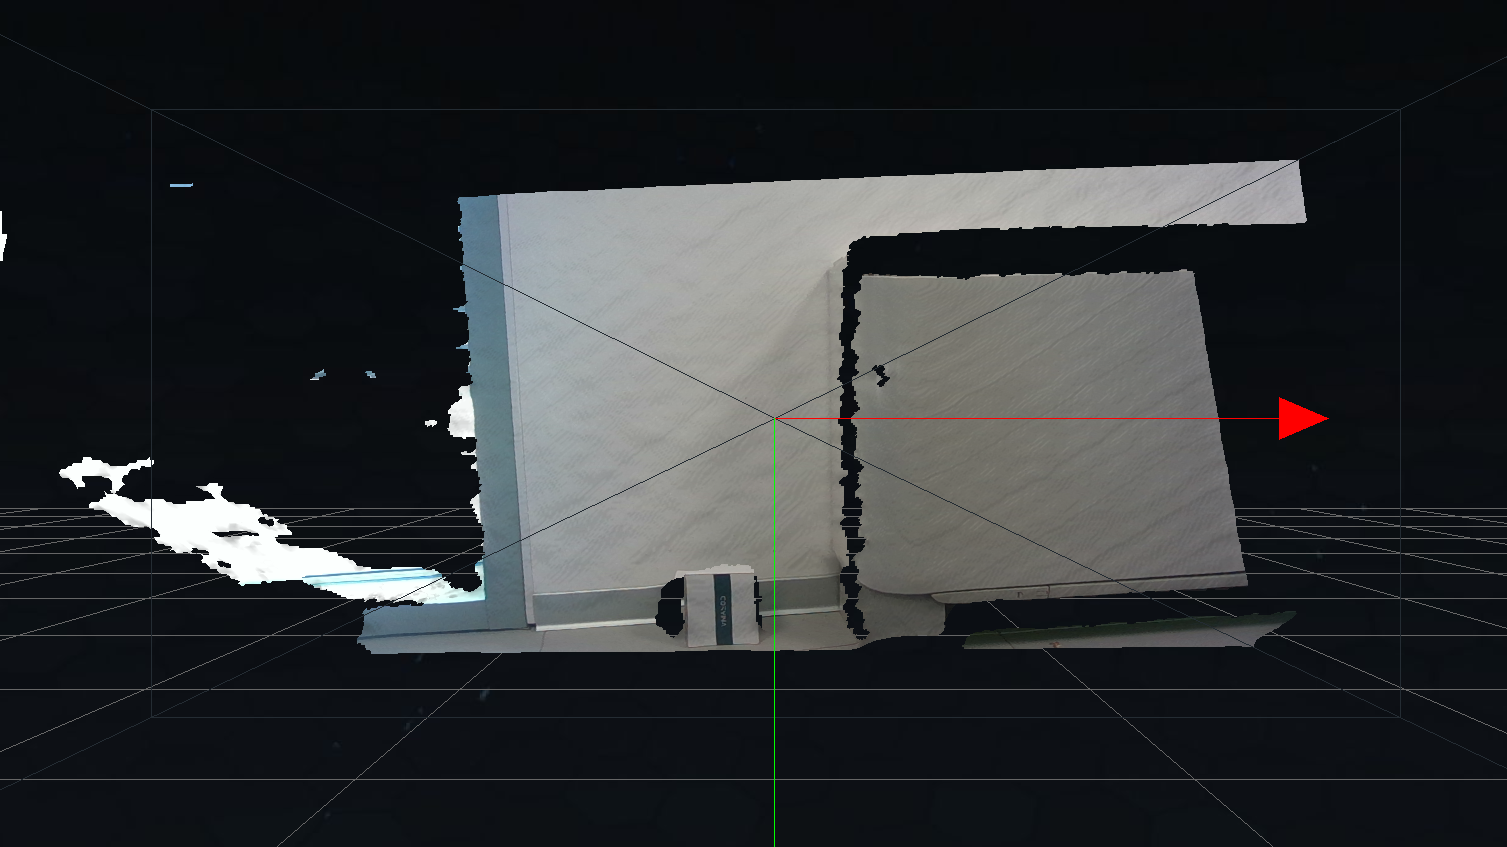
\includegraphics[width = 3in]{Images/Chapter 6/pcl2.png}}&
\subfloat[]{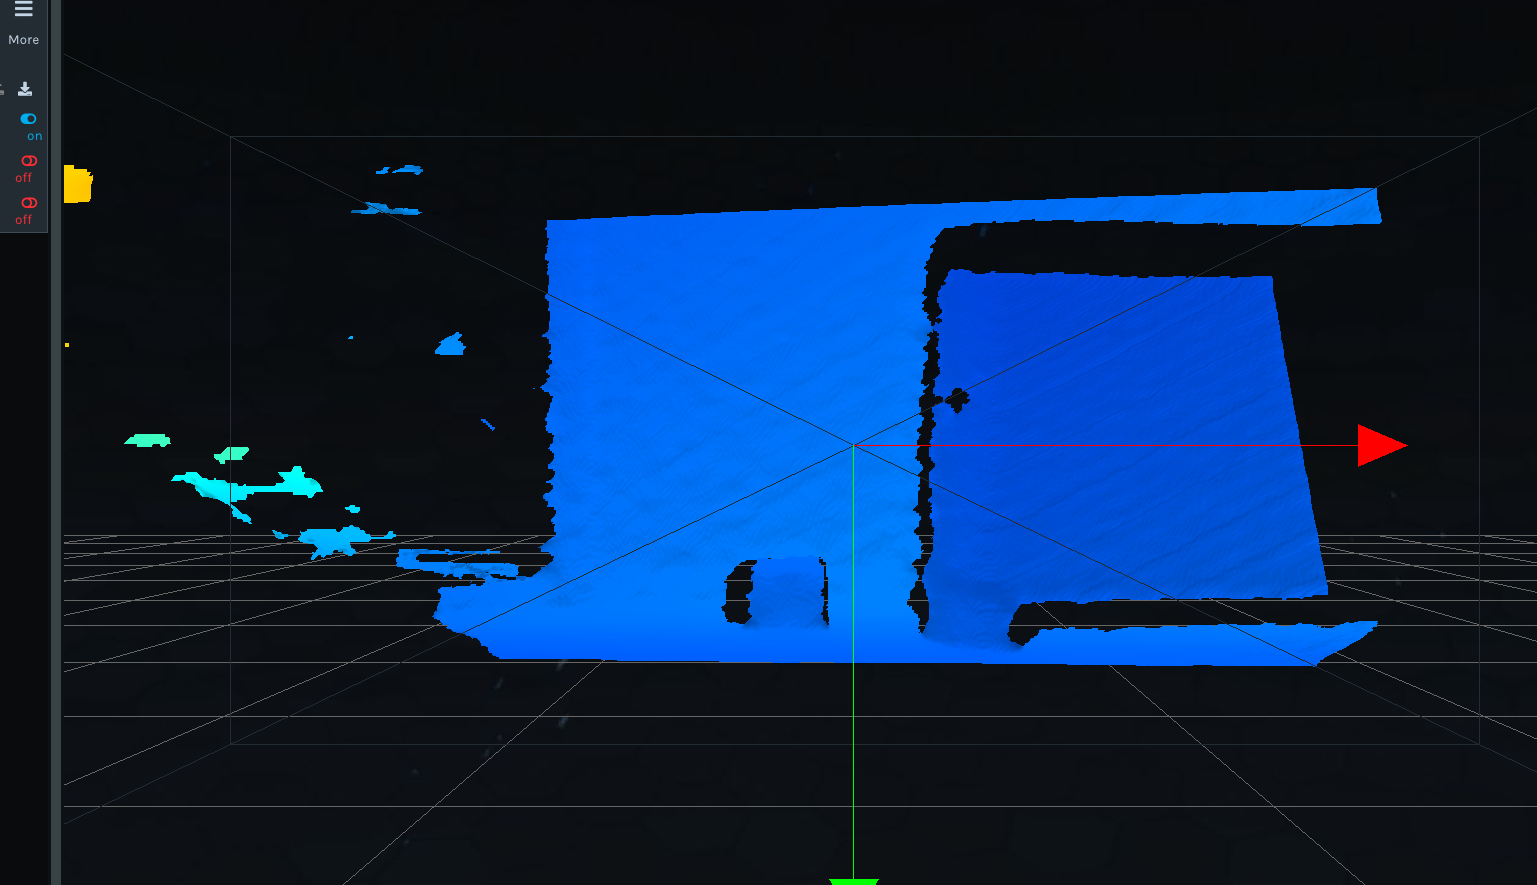
\includegraphics[width = 3in]{Images/Chapter 6/rgbd2.png}}
\end{tabular}
\caption{Pointcloud and RGB-D image visualization from Realsense SDK, taken from D455 camera}
\end{figure}
The sensor transmits the pointcloud data that are interpreted by ROS in a dedicated format.
The PointCloud2 object is an implementation of the \texttt{sensormsgs/PointCloud2} message type in ROS. The object contains meta-information about the message and the point cloud data. To access the actual data, use readXYZ to get the point coordinates and readRGB to get the color information, if available.
For the pointcloud use in ROS and visualization in RViz environment, two ROS nodes were set up: 
\begin{itemize}
    \item read: reads a point cloud from the camera sensor, publishing it as \texttt{sensor\_msgs/PointCloud2} message. This message contains a collection of N-dimensional points. The data may be in one dimension, so unordered, or in two dimensions, like images data are stored.
    \item write: subscribes to the topic \texttt{sensor\_msgs/PointCloud2} 
\end{itemize}

In order to manage pointcloud data, PCL library was adopted. The Point Cloud Library (PCL) is a standalone, large scale, open project for 2D/3D image and point cloud processing, that provides advanced methods for pointcloud data management and API integration. 
PCL makes us if a slightly different data class, pcl::PointCloud. This is the core point cloud class, though having a similar structure to that used in ROS, this enabling a straightforward conversion from PointCloud2 to PCL and viceversa. The motivation for this data class to exist stays in the fact that it enables nodes to work with individual data point as objects rather than with their raw data.
\section{Problem Explanation}
Part of the work at Oversonic Robotics involved testing the state of navigation, as seen in the previous chapter, in order to draw up useful reports both for internal benchmarking and to provide to customers.
During these tests, it was realised that, in certain particular indoor and/or outdoor environment conditions, the robot perceived phantom obstacles, which did not exist in reality.
This is critical as the objective for the robot's navigation is to perform the programmed path optimally and in the shortest possible time. It is therefore clear that if the local planner encounters these phantom obstacles, a great deal of time is lost and the robot travels a greater distance, also resulting in greater energy consumption.
It was therefore decided to devote time to identifying and solving this problem.
The conditions that encountered particular problems are: 
\begin{itemize}
    \item Reflective surfaces
    \item Tiled floor with highly repetitive patterns
\end{itemize}
In figure \ref{tiled_floor}, we can appreciate how the reflective zones of figure a are interpeted as dark areas in figure b, where it is shown RViz GUI.
\begin{figure}[H]
     \centering
     \subfloat[][a]{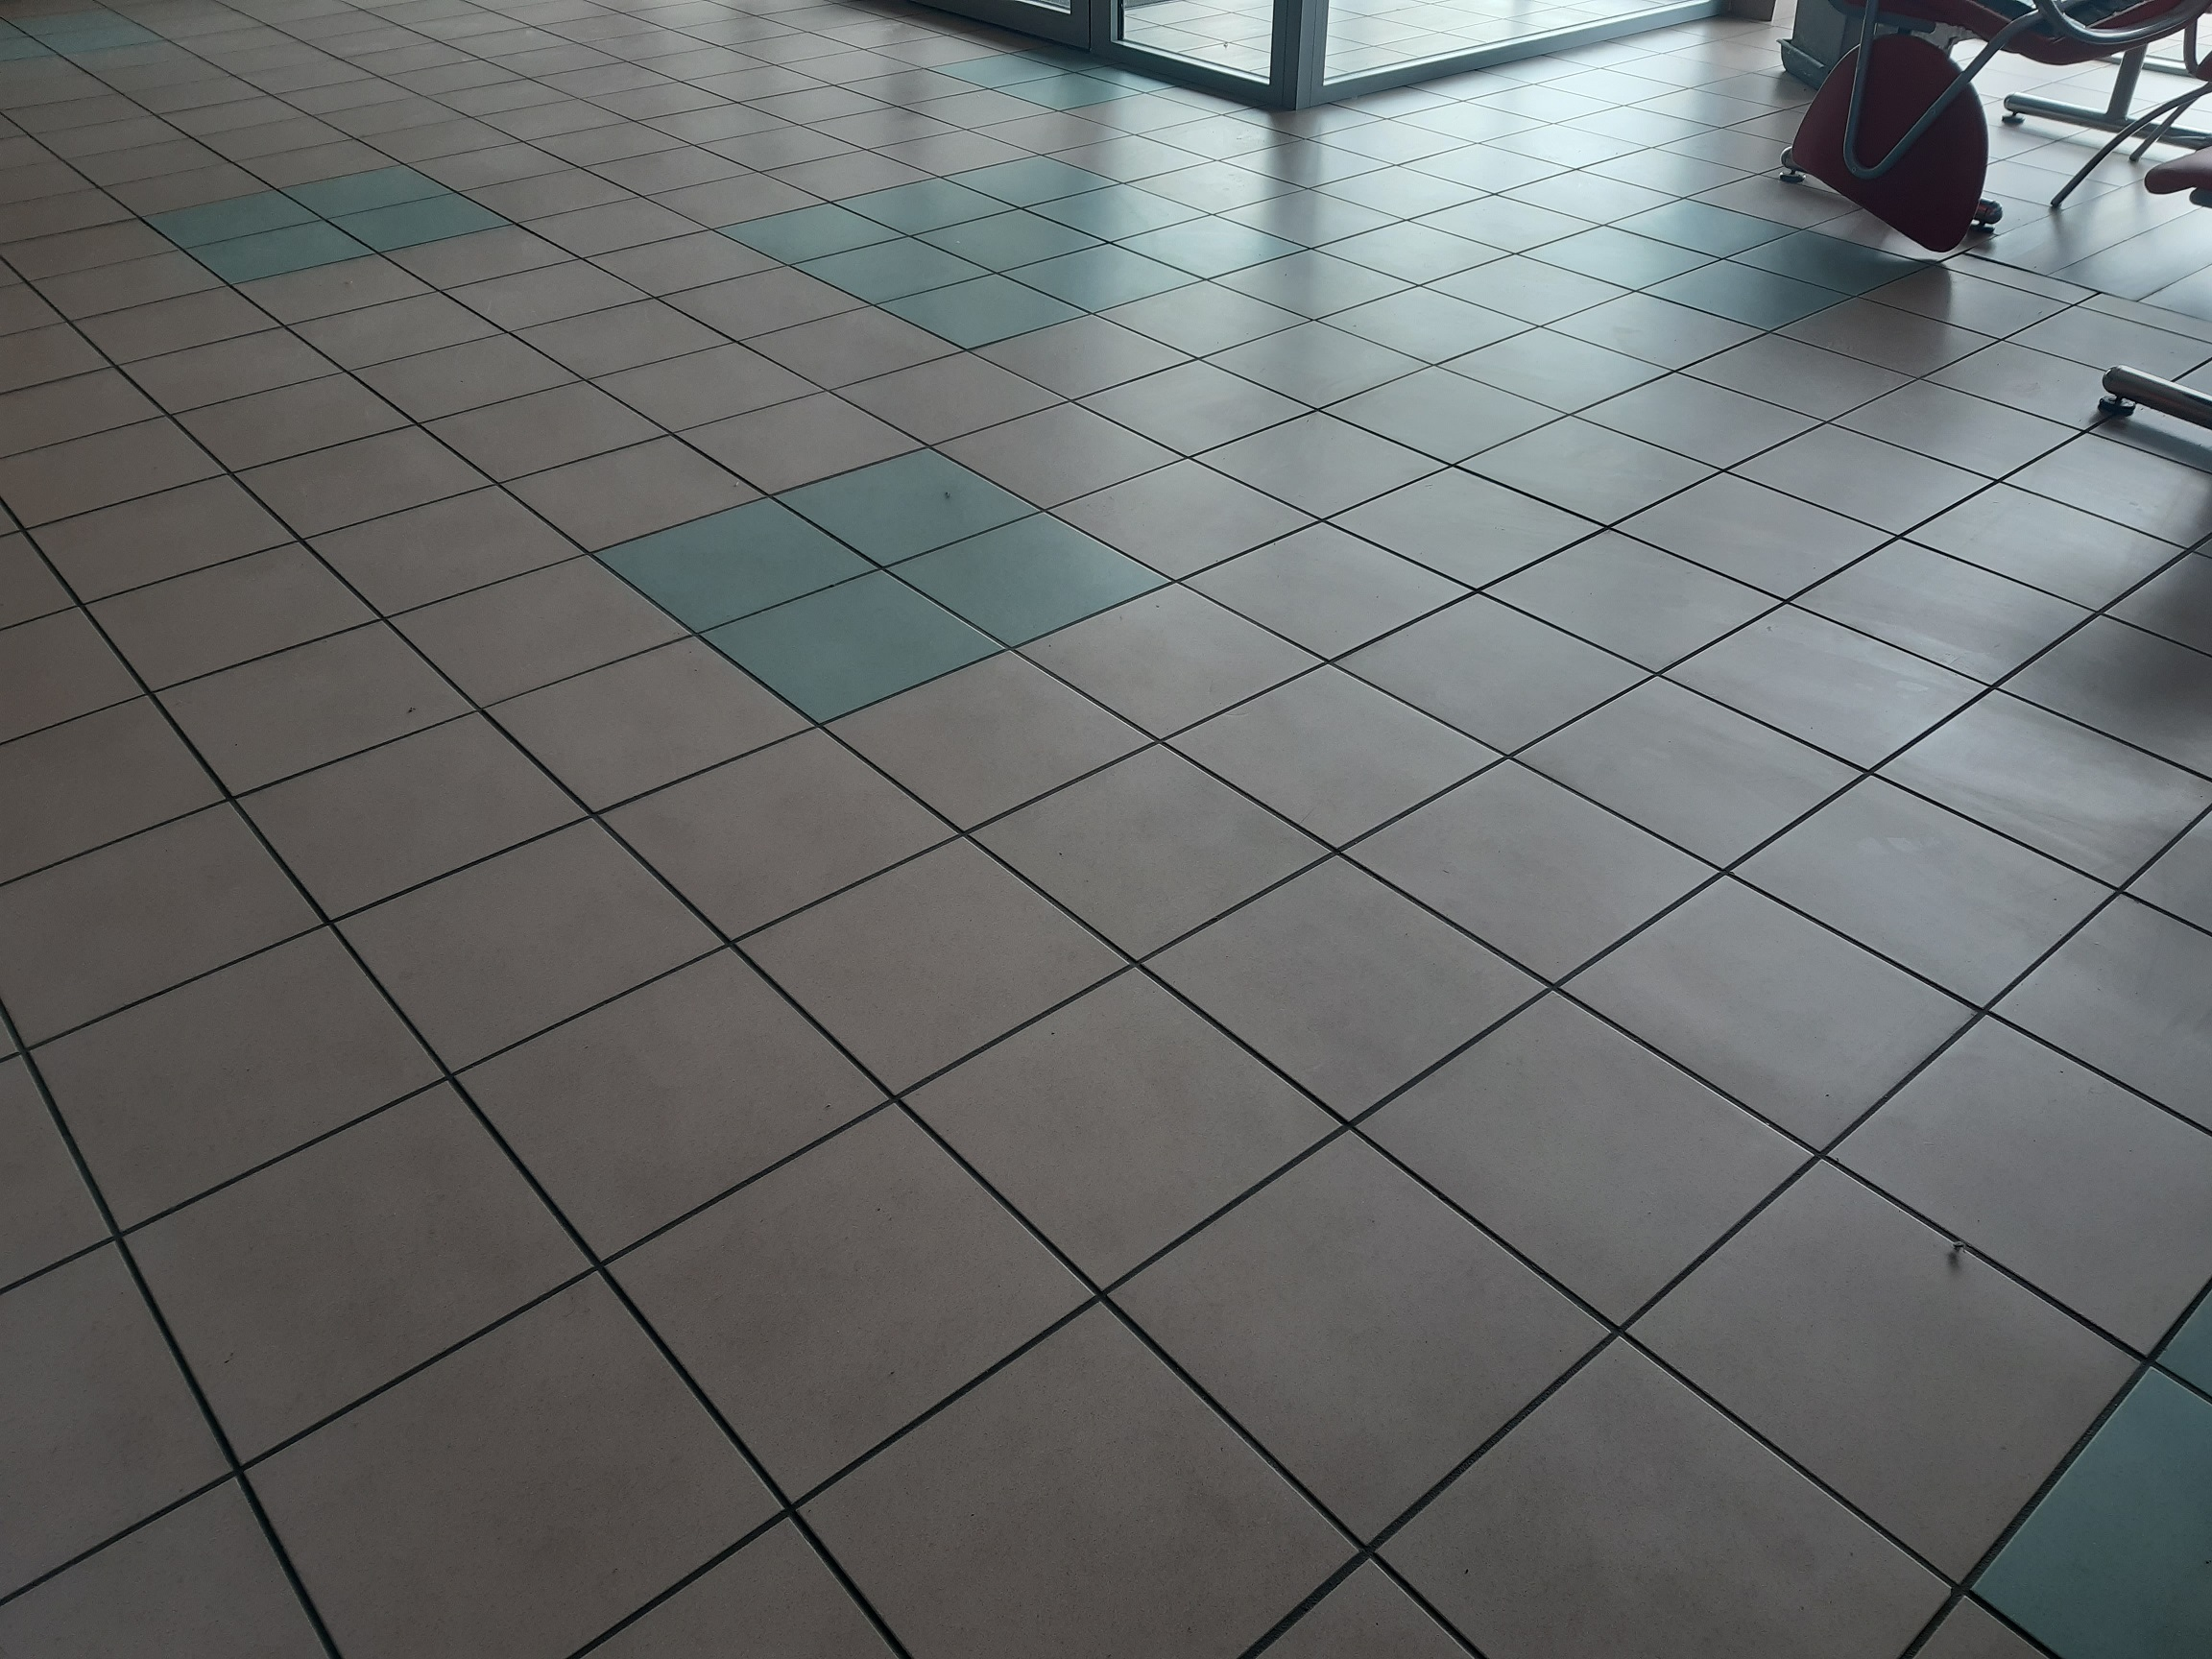
\includegraphics[scale=0.10]{Images/Chapter 6/tiledfloor.jpeg}\label{}}
     \hfill
     \subfloat[][b]{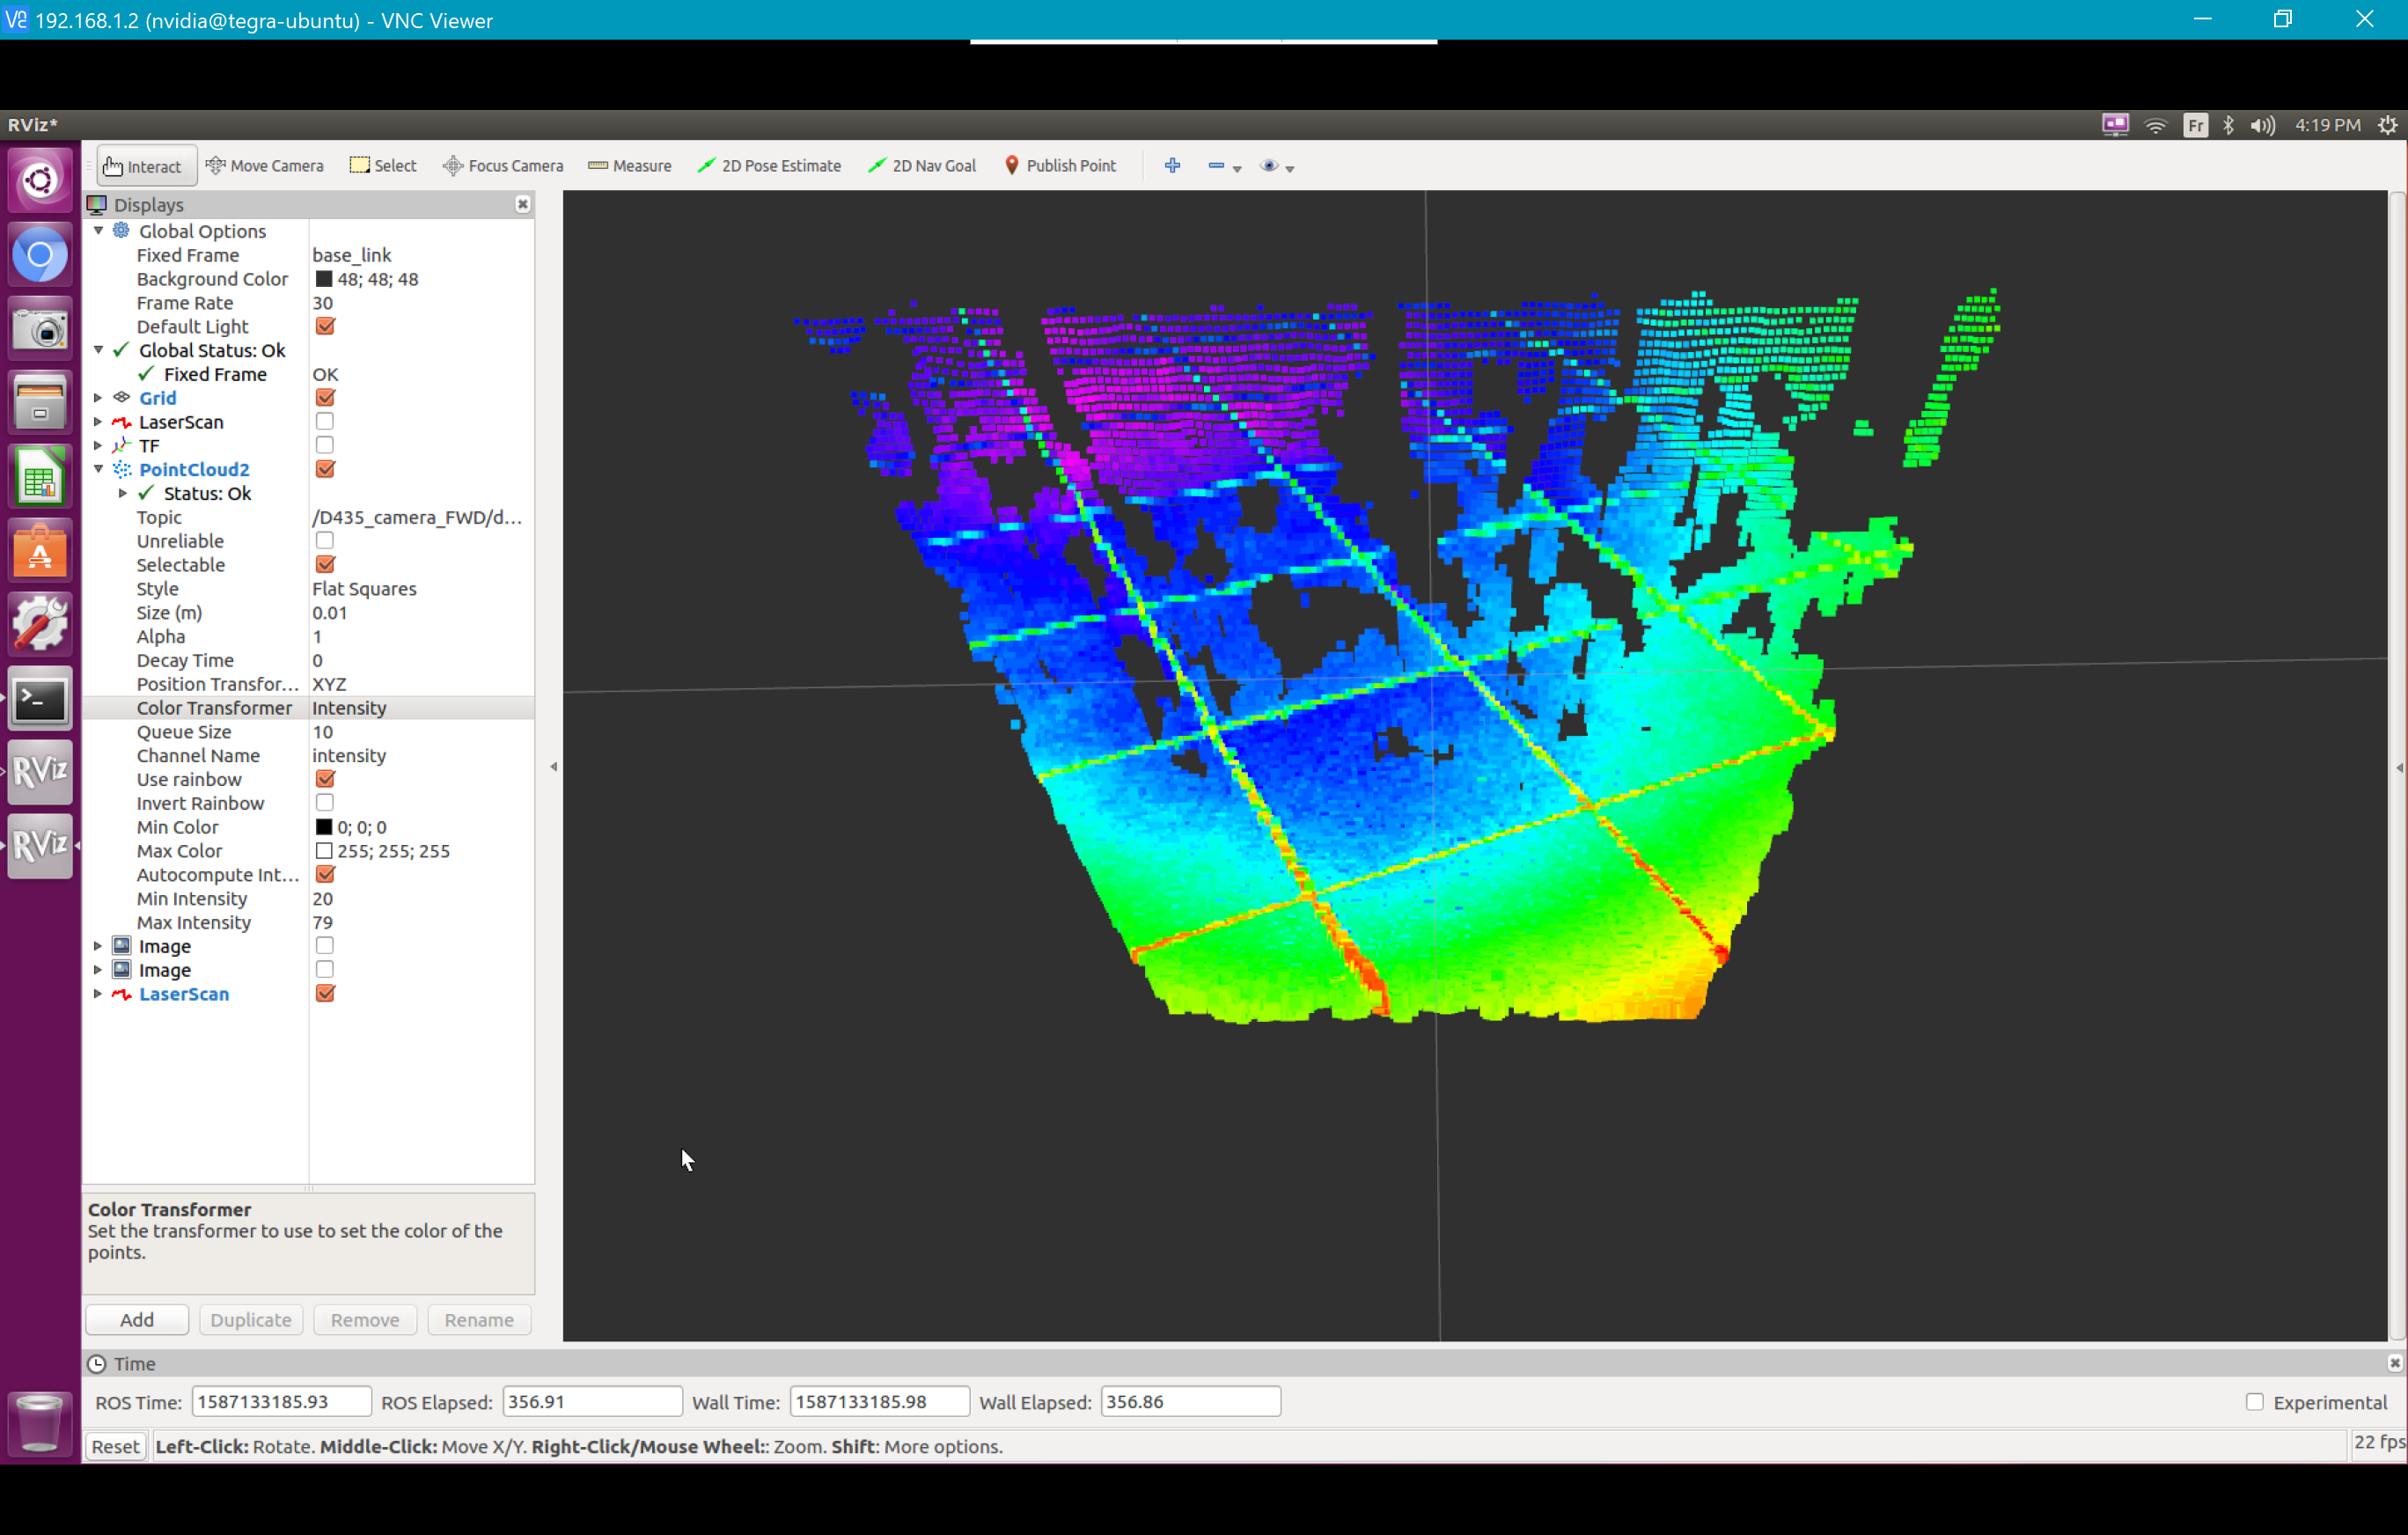
\includegraphics[scale=0.20]{Images/Chapter 6/tiledfloorrviz.png}\label{}}
     \caption{Visualization of the reflection issue experimented at Oversonic's office tiled floor}
     \label{tiled_floor}
\end{figure}

After careful research, it was discovered that many users of the intel realsense chambers were experiencing this problem but no solution was provided by Intel.
With the Intel RealSense D400 series of stereo depth cameras, depth is derived primarily from solving the correspondence problem between the simultaneously captured left and right video images, determining the disparity for each pixel (i.e. shift between object points in left vs right images), and calculating the depth map from disparity and triangulation.
The Depth RMS error that defines the depth noise for a localized plane fit to depth values can be defined as:
\begin{equation}
    Depth RMS error (mm) = \frac{Distance(mm)^2 \times Subpixel}{focal length(pixels) \times Baseline(mm)}
\end{equation}

Below is reported the findings for D455 RMS error:
\begin{center}
    

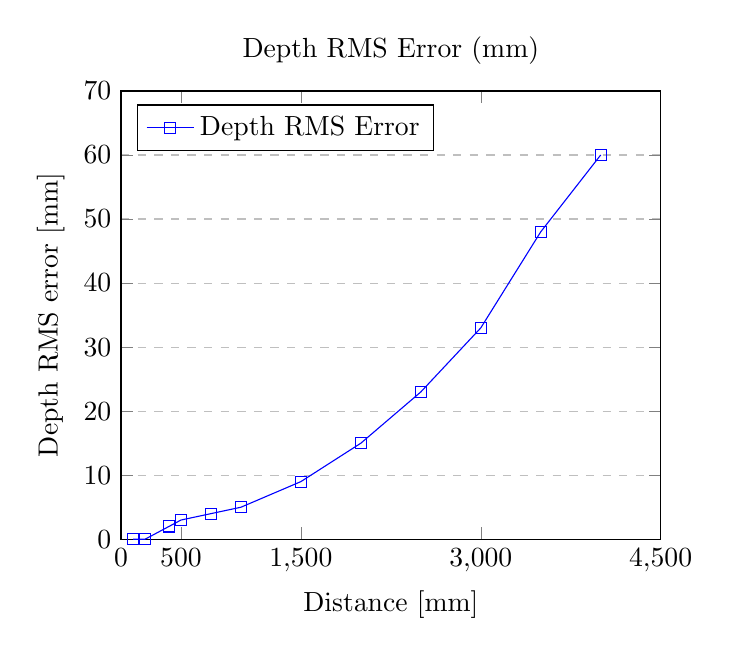
\begin{tikzpicture}[thick, scale=1]
\begin{axis}[
    title={Depth RMS Error (mm)},
    xlabel={Distance [mm]},
    ylabel={Depth RMS error [mm]},
    xmin=0, xmax=4500,
    ymin=0, ymax=70,
    xtick={0,500,1500,3000,4500},
    ytick={0,10,20,30,40,50,60, 70},
    legend pos=north west,
    ymajorgrids=true,
    grid style=dashed,
]

\addplot[
    color=blue,
    mark=square,
    ]
    coordinates {
    (100,0)(200,0)(400,2)(500,3)(750,4)(1000,5)(1500,9)(2000,15)(2500,23)(3000,33)(3500,48)(4000,60)
    };
    \legend{Depth RMS Error }
    
\end{axis}
\end{tikzpicture}
\end{center}
The  curve is obtained usind D455 with HFOV=90 deg, Xres=1280, baseline=50 mm and subpixel=0.08.
Initially, it was decided to try applying a polarising film to the outer lens of the camera.
In figure a polarizer is used to reduce the glare of sunlight reflecting off a window by only passing P-polarized light.
Polarizers indeed can be used to selectively attenuate different components of light in order to enhance human vision and photography. The motivation for the use of optical filters comes from Fresnel equations: by properly adopting the filter angulation at Brewster angle, all reflected S-light is polarized, so that all reflections are cancelled. Fresnel divided light into S- and P- polarization states, where S has the electric field normal to the plane of incidence and P has the electric field co planar with it.
Glare can lead to local saturation of portions of the image and false depth can result from objects partially reflected from the surface. Glare-induced saturation is usually associated with bright light sources such as sunlight or light bulbs. Reflection-related false depth typically occurs with textured objects reflected on shiny surfaces with little texture

\begin{figure}[H]
    \centering
    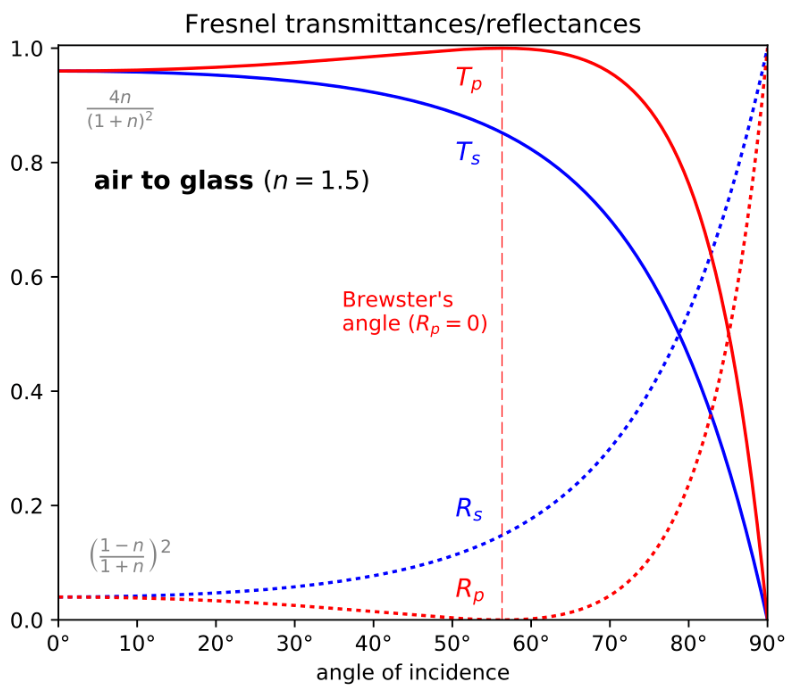
\includegraphics[scale=0.5]{Images/Chapter 6/glare.png}
    \caption{Fresnel transmittances/reflectances}
    \label{fig:my_label}
\end{figure}
Polarizers work well in condition of natural sunlight, as in figure \ref{fig:reflective_glass}, but in our working environment the optical filter showd no improvement on detecting ghost obstacles.

\begin{figure}[H]
    \centering
    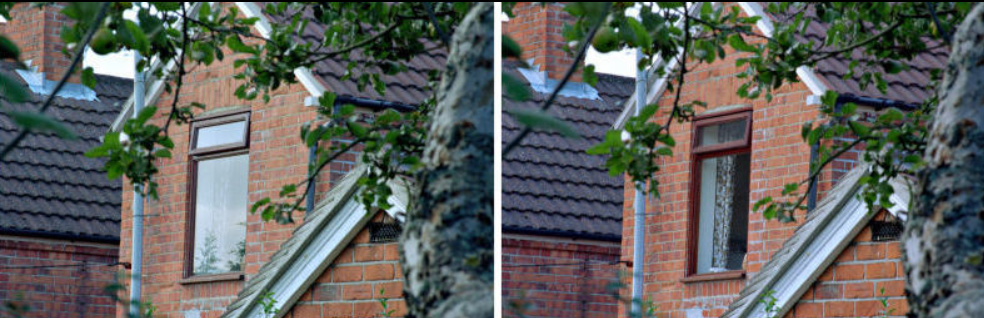
\includegraphics[scale = 0.5]{Images/Chapter 6/reflective_surface.png}
    \caption{On the right there is the image taken from D400 RealSense camera, on the left there is the image taken after applying the physical filter on the lens.}
    \label{fig:reflective_glass}
\end{figure}
In fact, even after applying the optical filter, the robot kept visualizing glare in form of black spaces, misleading obstacle detection.
In order to test the difference in performance with the application of the polarising film, a test identical to that already presented in Chapter \ref{ch:sim_test} was used.
In section \ref{section: experimentalpcl}, navigation metrics before and after film application can be appreciated.


\section{Proposed Solution}
Since the attempted solution by application of an optical filter led to only marginal improvements, it was decided to resort to a post-processing solution.
Intel RealSense SDK provides some buil-in methods to perform filtering, in particular:
\begin{itemize}
    \item Decimation: reduce resolution of depth frame
    \item Disparity: transformation between depth and disparity domains
    \item Spatial: edge-preserving smoothing
    \item Temporal: filter depth data by looking into previous frames
\end{itemize}
Promising results were achieved by applying these filters to saved file of pointcloud data, but this approach did not allow to perform real time filtering, so it was left for an online post-processing solution.
For this purpose, as already mentioned, the PCL library was used.
This library provides methods for filtering pointcloud data.
The approach was to treat ghost reflections as a mass of data too dense to be analysed and a statistical outlier removal filter was tried.
In fact, the idea behind it is to remove noisy measurements from the pointcloud, as these scattered outliers corrupt the results.
The solution therefore proposes statistical analysis around each point neighborhood: for every point compute the distance from the point itself to all of its neighbors.
A similar approach was proposed by \citet{Ning2018AnEO}:
The sparse pointcloud P is defined by N points such that $P = p_{1}, p_{2}, p_{3}, ..., p_{N}$ whereas the k nearest neighbor points of a point $p_{i}$ are defined as $KNN(p_{i})$, a set of k points such that $Q = q_{1}, q_{2}, q_{3}, ..., q_{k}$.
The algorithm removes points that are considered outliers based on geometric information.

The average geometric distance of a point $p_i$ from its neighbors is defined as:
\begin{equation}
 d_i = 1/k \sum_{j=1}^{k} dist(p_i,q_j)
\end{equation}
where dist(x,y) is a function that returns euclidean distance between two points. 
By assuming that the resulted distribution is Gaussian with a mean and a standard deviation, we can derive $\mu_d$ the overall mean distance and $\sigma_d$, the standard deviation of distances.
Hence, by tuning $\alpha$, the so-called standard deviation multiplier, we can define a threshold $T = \mu_d + \alpha \sigma_d$. 
Every point in the cloud, whose its kNN distance falls out of the interval defined by T, are directly discarded.
Tuning of $\alpha$ parameter was performed by trial and error.
Below is reported the resulting algorithm, algorithm \ref{alg:statistical}:

\begin{algorithm}
\caption{Statistical Outlier Removal: pure KNN approach}\label{alg:statistical}
\begin{algorithmic}
\STATE Set k
\STATE Set $\alpha$
\FOR{$P_i$ in input\_data}
    \STATE Locate kNN to point $P_i$
    \STATE Compute $d_i$ 
\ENDFOR
\STATE Compute $\mu_d$
\STATE Compute $\sigma_d$
\STATE Compute $T = \mu_d + \alpha \sigma_d$
\IF{$d_i$ > T}
\STATE Trim point $P_i$ from the pointcloud
\ENDIF
\end{algorithmic}
\end{algorithm}

The problem can be solved from another point of view that is by analyzing clusters of isolated pointcloud data, \citet{10.1371/journal.pone.0201280}.
Local density function, $LD(p_{i}$ of $p_{i}$ is introduced as:
\begin{equation}
    LD(p_{i}) = \frac{1}{k} \sum_{q_j \in KNN(p_i)} exp(\frac{-dist(p_i,q_j)}{d_i}
\end{equation}
The probability that a point belongs to outlier can be defined as $prob(p_i) = 1 - LD(p_i)$, where $prob(p_i) = 1 - LD(p_i)$ and it ranges between 0 and 1, so that a higher value means a higher probability for the point to be outlier.
The point $p_i$ is retained if it falls under some predefined threshold, like T in previous approach, so $prob(p_i) < \delta$.
The threshold is not intended to be universal, rather its value depends on its case of application.

\begin{algorithm}[H]
\caption{Statistical Outlier Removal: local density approach}\label{alg:statistical2}
\begin{algorithmic}
\STATE Set k
\STATE Set $\alpha$
\FOR{$P_i$ in input\_data}
    \STATE Locate kNN to point $P_i$
    \STATE Compute $LD(P_i)$
    \STATE Evaluate probability $prob(p_i)$
\ENDFOR
\STATE sort $prob(p_i)$ in ascending order
\IF{$prob(p_i)$ > $\delta$}
\STATE Trim point $P_i$ from the pointcloud
\ENDIF
\end{algorithmic}
\end{algorithm}

In figure \ref{fig:filt_scheme} the overall process flow is described. 
\begin{figure}[H]

    \centering
    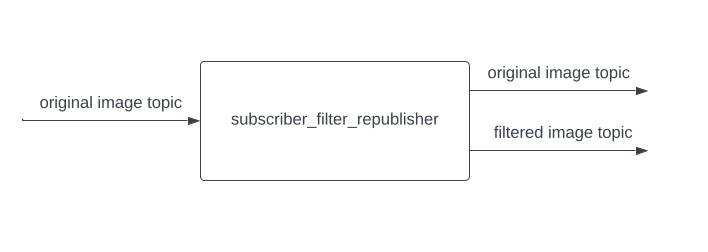
\includegraphics[scale=0.5]{Images/Chapter 6/filt_scheme.png}
    \caption{Overall process block scheme}
    \label{fig:filt_scheme}
\end{figure}
As initially stated, the goal of this filter is to perform online processing of point cloud. In our specific case, we want to take input data, perform the data transformations and then output both the filtered and original data, so that the user can choose which to keep.
Input data are transmitted from and to the ROStopic  \texttt{/d400\_lb/depth/color/points} through the subrscribe and publish paradigm. 
In order to work on the data with the PCL methods, it is necessary to transform the message structure from \texttt{PointCloud2} to PCL format and transform back to \texttt{PointCloud2} after the filtering has occured.
A crucial point for this approach is computing time, given the fact that we want the filter to process the data at real time.
It was necessary to provide an indication of the time required for the filter to elaborate the data, in order to understand its practical feasibility.
Initially, pre processing was made on the data and the filter was dealing with the entire amount of point cloud information at the same time. This led to an extremely high computing time (0.5 s) that is unacceptable for obstacle detection, in fact this brought to a further drop of navigation performance. 
It was thought that the problem was caused by a too strong filtering action, so we tried to decrease further the threshold.
This was a misconcept, since after a careful analysis it was discovered that the delay was introduced by the conversion of data format from PointCLoud2 to PCL format. 
The only solution left at this point was to try and pre-process the data using a decimation filter, in order to feed the code with the least required amount of data.
Decimation filter is has been designed by Intel RealSense to effectively reduce the depth scene complexity. The filter run on kernel sizes [2x2] to [8x8] pixels. For patches sized 2 and 3 the median depth value is selected. For larger kernels, 4-8 pixels, the mean depth is used due to performance considerations, \citet{intelrealsense}.
In order to understand which configuration worked better inside the computational time constraint, several tests were conducted.
In table \ref{tab: avg_comp_time} average results are reported, key indicators are:
\begin{itemize}
    \item Converting Time represents the 2-way cost of converting data: from PointCloud2 to PCL and from PCL back to PointCloud2
    \item Processing Time represents the computational cost of performing the statistical outlier removal on the input cloud
\end{itemize}

\begin{table}[H]
\centering
\begin{tabular}{|l|c|c|c|}
\hline
\rowcolor[HTML]{FFFFFF} 
\textbf{Configuration}                                                         & \textbf{Converting Time {[}s{]}} & \textbf{Processing Time  {[}s{]}} & \textbf{ Total Time {[}s{]}} \\ \hline
\rowcolor[HTML]{FFFFFF} 
\begin{tabular}[c]{@{}l@{}}Pre-filter: none\\ Filter: K=50\end{tabular}        & 0.42                                  & \cellcolor[HTML]{FFFFFF}0.13           & 0.55                             \\ \hline
\rowcolor[HTML]{FFFFFF} 
\begin{tabular}[c]{@{}l@{}}Pre-filter: none\\ Filter: K=9\end{tabular}         & 0.25                                  & 0.09                                   & \cellcolor[HTML]{FFFFFF}0.34     \\ \hline
\rowcolor[HTML]{FFFFFF} 
\begin{tabular}[c]{@{}l@{}}Pre-filter: decimation\\ Filter: K= 50\end{tabular} & 0.07                                  & 0.03                                   & \cellcolor[HTML]{FFFFFF}0.10     \\ \hline
\rowcolor[HTML]{FFFFFF} 
\begin{tabular}[c]{@{}l@{}}Pre-filter: decimation\\ Filter: K= 9\end{tabular}  & 0.04                                  & 0.01                                   & \cellcolor[HTML]{FFFFFF}0.05     \\ \hline
\end{tabular}
\caption{Comparison of average computational times implied by different filter - prefilter configurations}
\label{tab: avg_comp_time}
\end{table}

This data was collected and analysed by running the code on a camera detached from the robot. Once the configurations to be tested had been chosen, the physical robot was moved on. The idea was to define an initial benchmark, obtained from chapter \ref{ch:sim_test}, and to collect useful data to compare the same metrics with the chosen configurations. The aim was to analytically assess whether and to what extent the various configurations could improve the management of phantom reflections and the performance of navigation in general.
\begin{figure}[H]
     \centering
     \subfloat[Image from the original pointcloud topic][a]{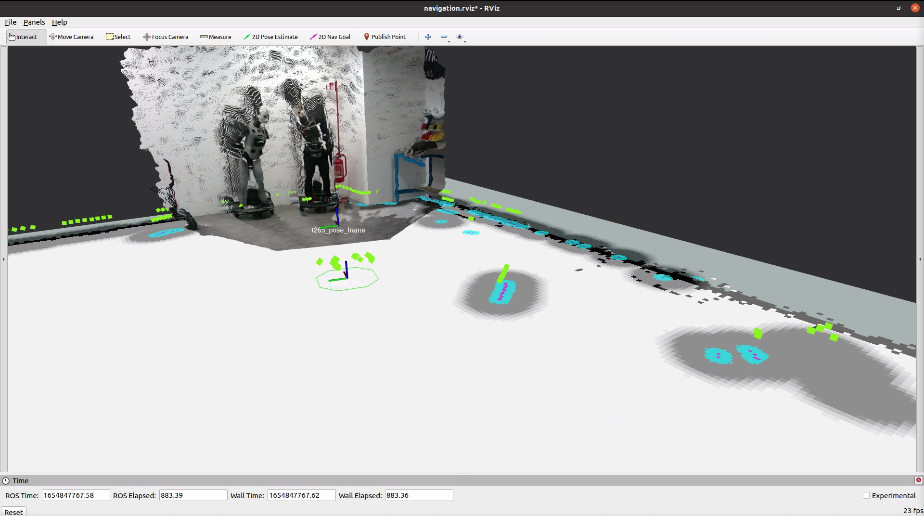
\includegraphics[scale=0.4]{Images/Chapter 6/pcloriginalimage.png}\label{}}
     \hfill
     \subfloat[Image from the filtered pointcloud topic][b]{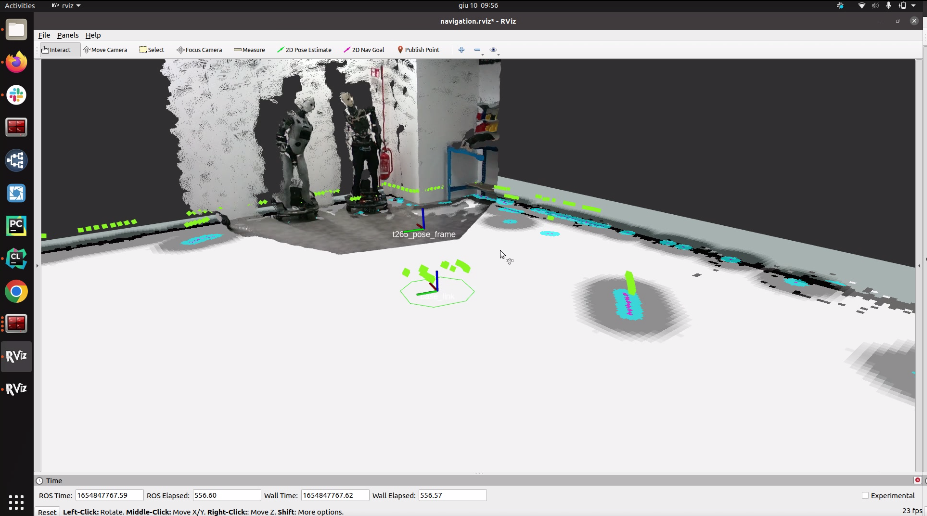
\includegraphics[scale=0.4]{Images/Chapter 6/pclfilteredimage.png}\label{}}
     \caption{Pre and post filtering comparison}
     \label{tiled_floor}
\end{figure}.
\newpage
Overall, the designed process flow resulted as reported in algorithm:
\ref{alg:postprocesser}:

\begin{algorithm}[H]
\caption{Postprocesser}\label{alg:postprocesser}
\begin{algorithmic}
\STATE Set magnitude of decimation filter
\STATE Set k
\STATE Set $\alpha$
\STATE Subscribe pointcloudtopic
\STATE Input\_data: pointcloud topic
\FOR{$P_i$ in input\_data}
    \STATE Convert from PointCloud2 to PCL::cloud
    \STATE Locate kNN to point $P_i$
    \STATE Compute $d_i$ 
\ENDFOR
\STATE Compute $\mu_d$
\STATE Compute $\sigma_d$
\STATE Compute $T = \mu_d + \alpha \sigma_d$
\IF{$d_i$ > T}
\STATE Trim point $P_i$ from cloud
\ENDIF
\STATE Output\_data = cloud
\FOR{$P_i$ in cloud}
    \STATE Convert from PCL to PointCloud2
\ENDFOR
\STATE publish pointcloud topic and pointcloud\_filtered topic
\end{algorithmic}
\end{algorithm}

The complete code written in C++ can be found in appendix \ref{ch:appB}. 
\section{Experimental Results}
\label{section: experimentalpcl}
In order to assess what impact the introduction of the pointcloud filter had, the N002 robot was subjected to a test session on the same path used in the chapter \ref{ch:sim_test}. Of the various configurations tested, only the most significant are presented below for conciseness. All configurations were tested five times, under the same lighting conditions, in order to ensure the comparability of the results. Stuck time is introduced.
\subsection{Starting configuration: no pointcloud filter, no prefilter}
\begin{table}[H]
\centering
\resizebox{\columnwidth}{!}{%
\begin{tabular}{|c|c|c|c|c|c|}
\hline
\textbf{\begin{tabular}[c]{@{}c@{}}Nav Avg Speed\\ {[}m/s{]}\end{tabular}} &
  \textbf{\begin{tabular}[c]{@{}c@{}}Mov Fw Avg Speed\\ {[}m/s{]}\end{tabular}} &
  \textbf{\begin{tabular}[c]{@{}c@{}}Rot Avg Speed\\ {[}m/s{]}\end{tabular}} &
  \textbf{\begin{tabular}[c]{@{}c@{}}Nav Time\\ {[}s{]}\end{tabular}} &
  \textbf{\begin{tabular}[c]{@{}c@{}}Rotating Time\\ {[}s{]}\end{tabular}} &
  \textbf{\begin{tabular}[c]{@{}c@{}}Stuck Time\\ {[}s{]}\end{tabular}} \\ \hline
0.44 & 0.5  & 0.61 & 56.79 & 6.35 & 0.23 \\ \hline
0.46 & 0.52 & 0.63 & 53.69 & 4.44 & 0.33 \\ \hline
0.46 & 0.51 & 0.64 & 53.79 & 3.94 & 0.12 \\ \hline
0.45 & 0.51 & 0.63 & 54.14 & 3.94 & 0.41 \\ \hline
0.46 & 0.51 & 0.66 & 53.99 & 3.9  & 0.11 \\ \hline
\end{tabular}%
}
\caption{Measurements with original set up}
\label{tab:dataoriginalsetup}
\end{table}


\subsection{Pointcloud filter with K=9, no prefilter}
\begin{table}[H]
\centering
\resizebox{\columnwidth}{!}{%
\begin{tabular}{|c|c|c|c|c|c|}
\hline
\textbf{\begin{tabular}[c]{@{}c@{}}Nav Avg Speed\\ {[}m/s{]}\end{tabular}} &
  \textbf{\begin{tabular}[c]{@{}c@{}}Mov Fw Avg Speed\\ {[}m/s{]}\end{tabular}} &
  \textbf{\begin{tabular}[c]{@{}c@{}}Rot Avg Speed\\ {[}m/s{]}\end{tabular}} &
  \textbf{\begin{tabular}[c]{@{}c@{}}Nav Time\\ {[}s{]}\end{tabular}} &
  \textbf{\begin{tabular}[c]{@{}c@{}}Rotating Time\\ {[}s{]}\end{tabular}} &
  \textbf{\begin{tabular}[c]{@{}c@{}}Stuck Time\\ {[}s{]}\end{tabular}} \\ \hline
0.45 & 0.5  & 0.65 & 55    & 4.52 & 0.11 \\ \hline
0.45 & 0.5  & 0.63 & 54.6  & 4.5  & 0.1  \\ \hline
0.46 & 0.51 & 0.65 & 53.69 & 4.81 & 0.01 \\ \hline
0.46 & 0.51 & 0.64 & 54.09 & 5.61 & 0.19 \\ \hline
0.46 & 0.52 & 0.61 & 52.89 & 5.35 & 0.11 \\ \hline
\end{tabular}%
}
\caption{Pointcloud filter k=9, no prefilter}
\label{tab:pclnoprefilt}
\end{table}

\subsection{Pointcloud filter with K=9, decimation prefilter}
\begin{table}[H]
\centering
\resizebox{\columnwidth}{!}{%
\begin{tabular}{|c|c|c|c|c|c|}
\hline
\textbf{\begin{tabular}[c]{@{}c@{}}Nav Avg Speed\\ {[}m/s{]}\end{tabular}} &
  \textbf{\begin{tabular}[c]{@{}c@{}}Mov Fw Avg Speed\\ {[}m/s{]}\end{tabular}} &
  \textbf{\begin{tabular}[c]{@{}c@{}}Rot Avg Speed\\ {[}m/s{]}\end{tabular}} &
  \textbf{\begin{tabular}[c]{@{}c@{}}Nav Time\\ {[}s{]}\end{tabular}} &
  \textbf{\begin{tabular}[c]{@{}c@{}}Rotating Time\\ {[}s{]}\end{tabular}} &
  \textbf{\begin{tabular}[c]{@{}c@{}}Stuck Time\\ {[}s{]}\end{tabular}} \\ \hline
0.46 & 0.52 & 0.61 & 53.49 & 5.13 & 0.033 \\ \hline
0.46 & 0.52 & 0.59 & 53.19 & 5.5  & 0.035 \\ \hline
0.47 & 0.53 & 0.64 & 52.39 & 4.92 & 0.052 \\ \hline
0.46 & 0.52 & 0.65 & 53.6  & 5.52 & 0.081 \\ \hline
0.46 & 0.52 & 0.6  & 52.8  & 4.92 & 0.061 \\ \hline
\end{tabular}%
}
\caption{Pointcloud filter K=9, decimation filter}
\label{tab:pcl}
\end{table}
\newpage
\section{Comments}
In reporting the measurements from these tests, the focus was on the statistics on the average linear and angular velocities of navigation and the times the robot remained in the predefined states.
In order to assess the improvements made, particular attention should be paid to the Navigation and Stuck time values. These in fact come into play when the robot recognises obstacles to be overcome and consequently, increase in value. It can be seen that the initial configuration presents average navigation and stuck times of 54.48 s and 0.24 s respectively. By inserting the pointcloud filter with a filter power dictated by K=9, the values drop to 54.05 s and 0.104 s. Since the computation time still proved to be high, i.e. one tenth of a second, it was decided to try prefiltering the incoming data to the filter in order to lighten the amount of data to be analysed. The results were promising, leading to a browsing time of 53.1 s and a stuck time of 0.052 s, at the cost of an average computation time of 0.05 s. These differences may seem marginal, but when transported in the context of the use of many working hours, they take on a non-negligible importance. The inclusion of the pointcloud filter has also resulted in a more continuous navigation that allows the robot to reach its objectives in less time and avoiding discontinuities in movements that can accelerate wear and tear in the long run.